\chapterhead{CHƯƠNG 4 $-$ KẾT QUẢ HỆ THỐNG MẠNG}
\addcontentsline{toc}{chapter}{CHƯƠNG 4 $-$ KẾT QUẢ HỆ THỐNG MẠNG} 
\section*{4.1 Kiểm tra hệ thống và đánh giá}
\addcontentsline{toc}{section}{4.1 Kiểm tra hệ thống và đánh giá}
\subsubsection{Cấu hình VLAN và Trunking}
\begin{figure}[h]
			\subfloat[Cấu hình VLAN trên Core\label{fig:Pic_22}]
			{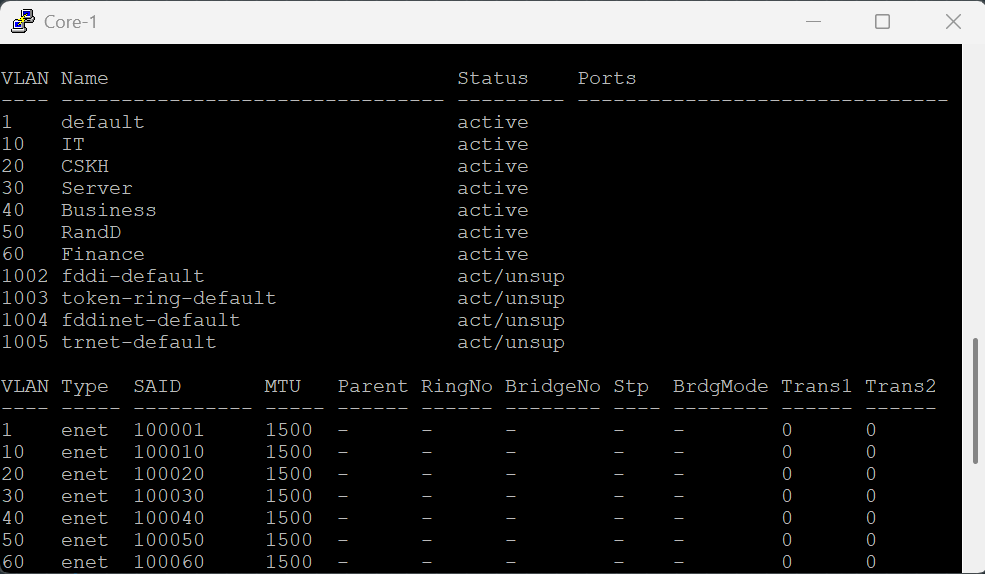
\includegraphics[width=7cm]{img/VLAN_CORE1.png}}\hfill
			\subfloat[Cấu hình VLAN trên Leaf\label{fig:Pic_23}]
			{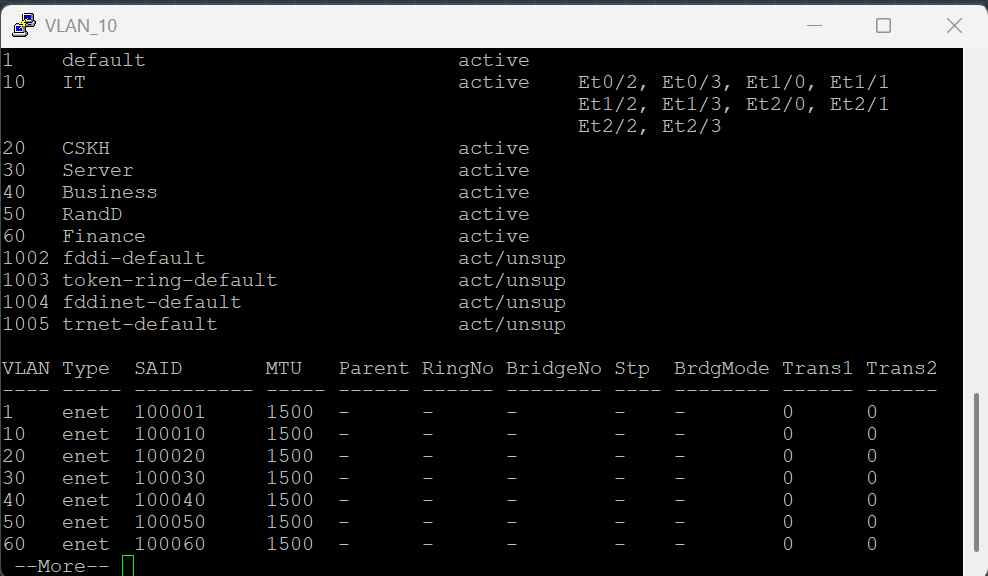
\includegraphics[width=7cm]{img/VLAN_LEAF1.png}}\hfill
			\caption{Xem cấu hình VLAN}
			\label{fig:Pic_1111}
\end{figure}
\begin{figure}[H]
			\subfloat[Cấu hình Trunking trên Core\label{fig:Pic_22}]
			{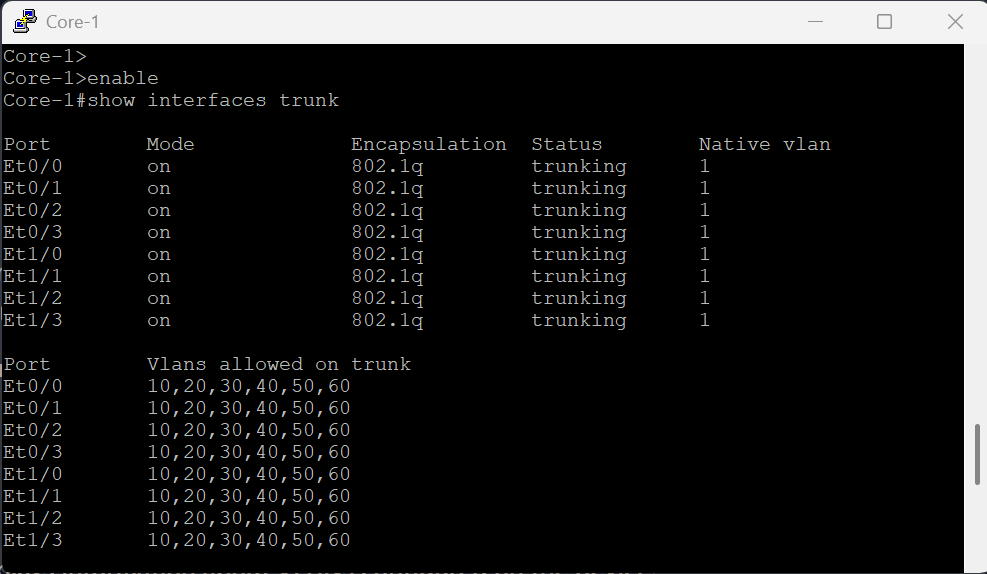
\includegraphics[width=7cm]{img/TRUNKING_CORE1.png}}\hfill
			\subfloat[Cấu hình Trunking trên Leaf\label{fig:Pic_23}]
			{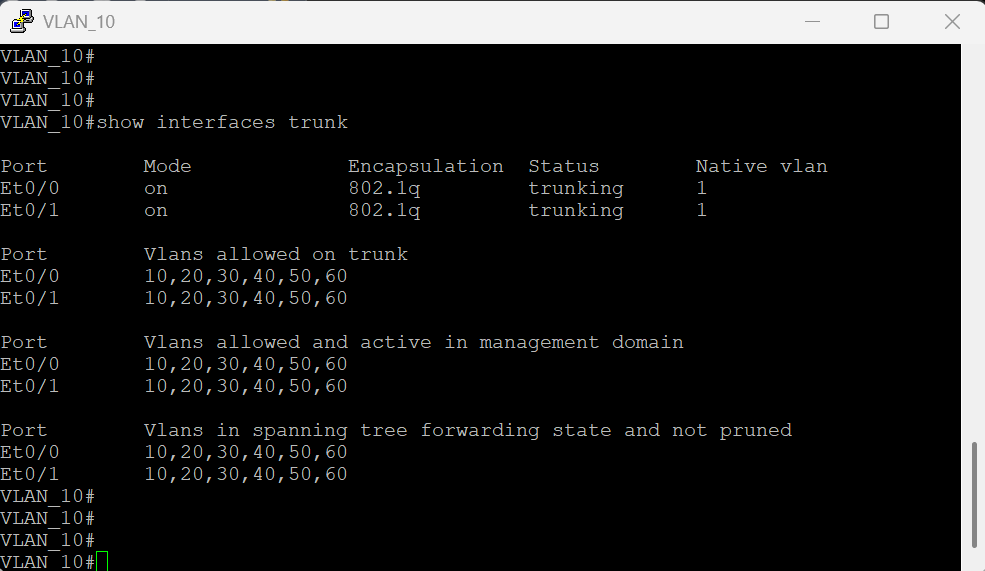
\includegraphics[width=7cm]{img/TRUNKING_LEAF1.png}}\hfill
			\caption{Xem cấu hình Trunking}
			\label{fig:Pic_1112}
\end{figure}
\subsubsection{Xem cây Spanning-tree}
\begin{figure}[H]
			\subfloat[Xem của VLAN 10 trên CORE-1\label{fig:Pic_22}]
			{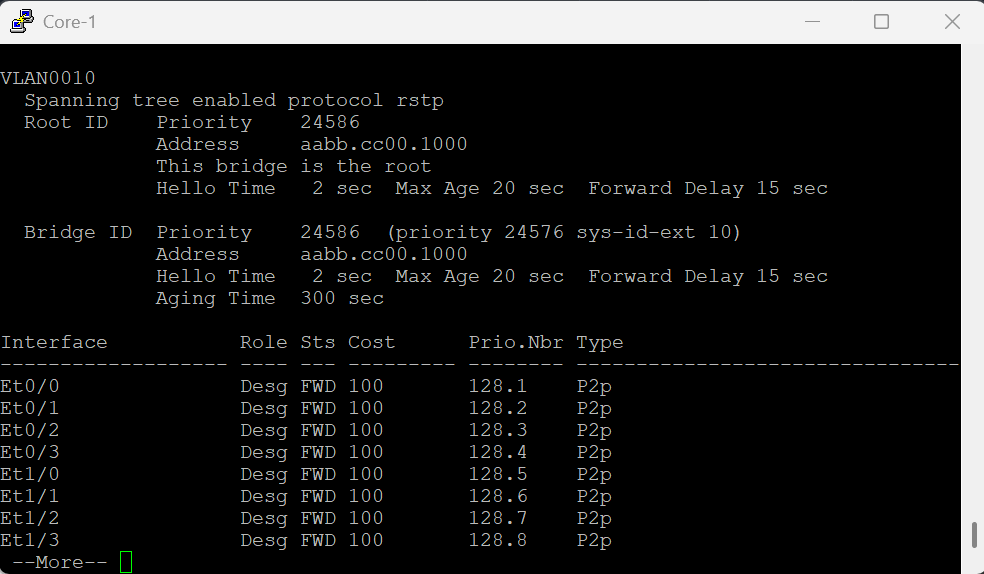
\includegraphics[width=7cm]{img/SPANTREEVL10Core1.png}}\hfill
			\subfloat[Xem của VLAN 10 trên CORE-2\label{fig:Pic_23}]
			{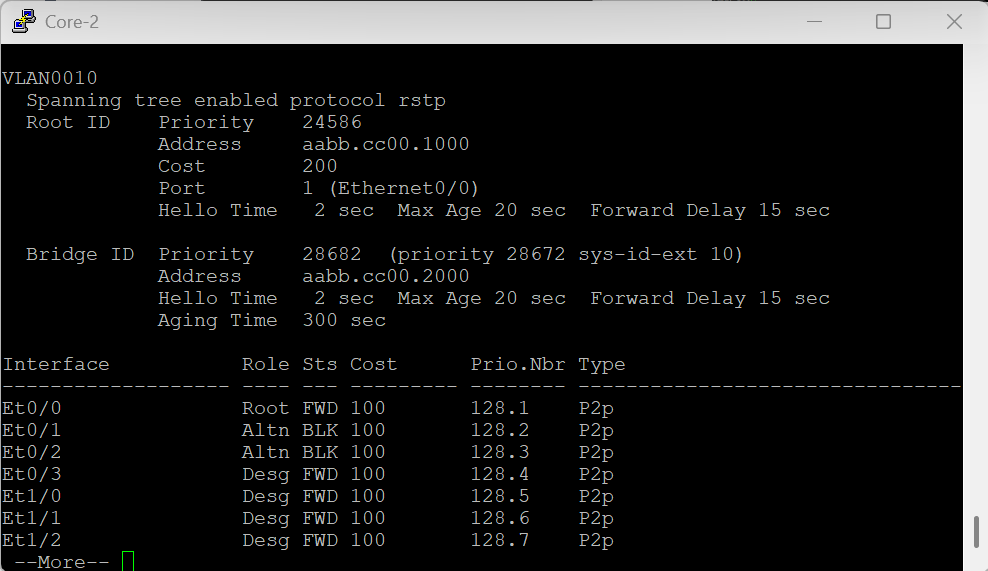
\includegraphics[width=7cm]{img/SPANTREEVL10Core2.png}}\hfill
			\caption{Xem hội tụ Spanning-tree VLAN 10}
			\label{fig:Pic_1113}
\end{figure}
\begin{figure}[H]
			\subfloat[Xem của VLAN 40 trên CORE-1\label{fig:Pic_22}]
			{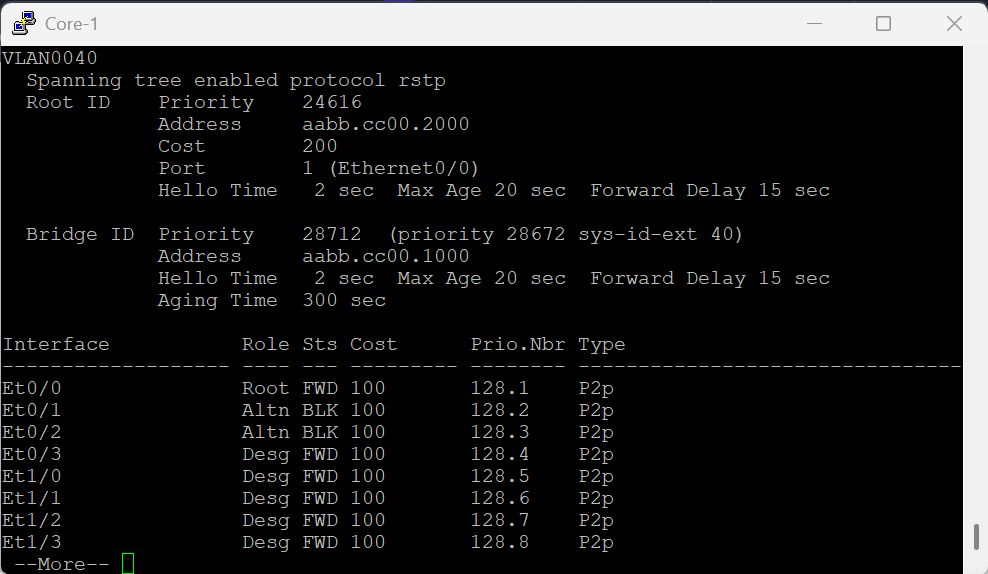
\includegraphics[width=7cm]{img/SPANTREEVL40Core1.png}}\hfill
			\subfloat[Xem của VLAN 40 trên CORE-2\label{fig:Pic_23}]
			{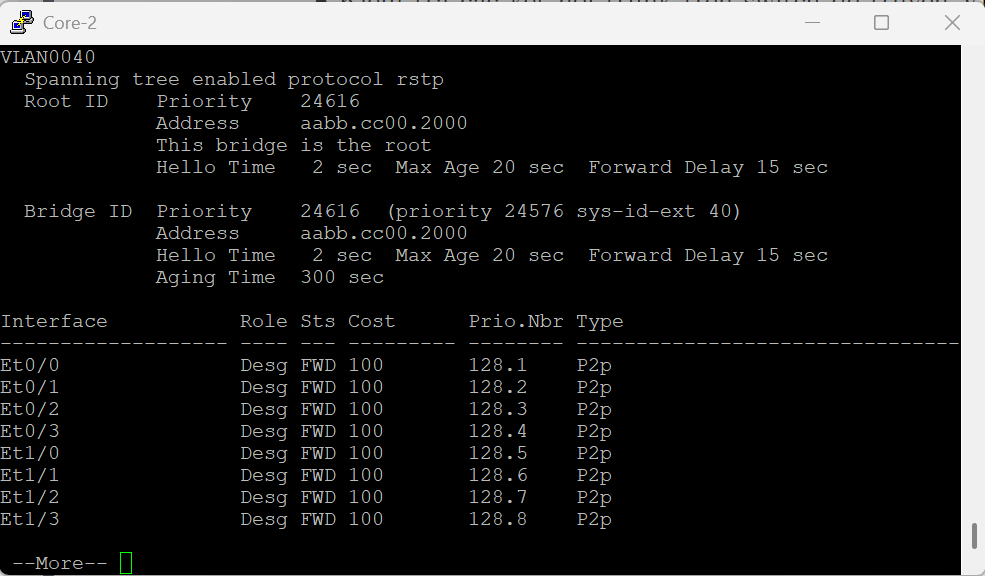
\includegraphics[width=7cm]{img/SPANTREEVL40Core2.png}}\hfill
			\caption{Xem hội tụ Spanning-tree VLAN 40}
			\label{fig:Pic_1113}
\end{figure}
\subsubsection{Xem IP VLAN và VRRP}
\begin{figure}[H]
			\subfloat[IP VLAN và VRRP trên CORE-1\label{fig:Pic_22}]
			{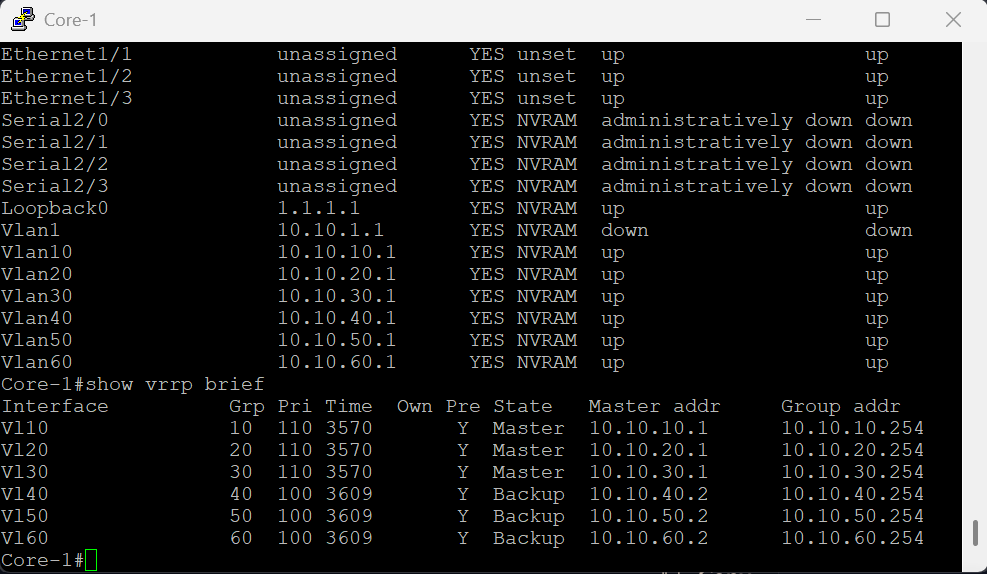
\includegraphics[width=7cm]{img/IP_VRRPCore1.png}}\hfill
			\subfloat[IP VLAN và VRRP trên CORE-2\label{fig:Pic_23}]
			{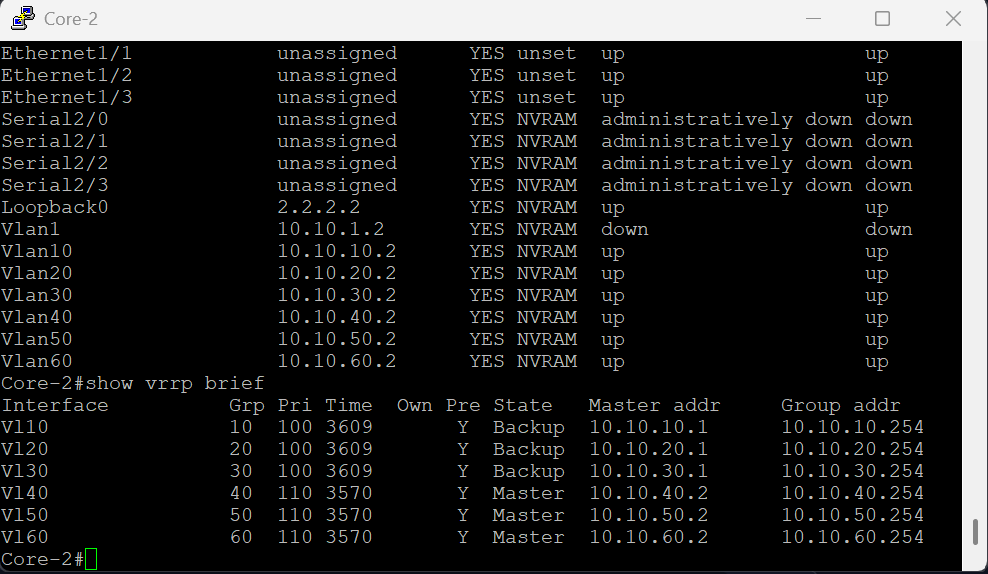
\includegraphics[width=7cm]{img/IP_VRRPCore2.png}}\hfill
			\caption{Xem thông tin IP VLAN và VRRP}
			\label{fig:Pic_1113}
\end{figure}
\subsubsection{Xem thông tin DHCP}
\begin{figure}[H]
			\subfloat[DHCP Serive trên CORE-1\label{fig:Pic_22}]
			{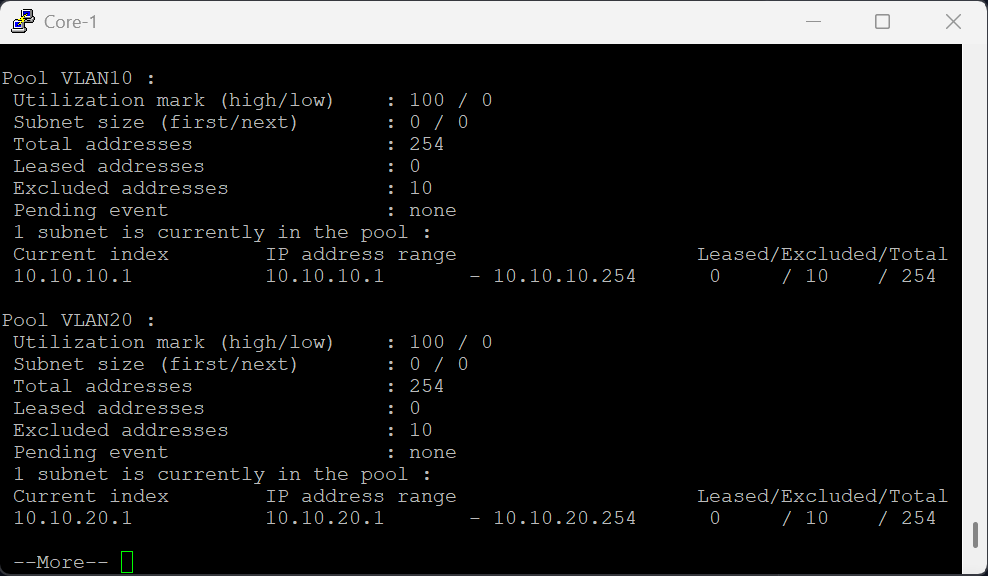
\includegraphics[width=7cm]{img/DHCP_CORE1.png}}\hfill
			\subfloat[DHCP Service trên CORE-2\label{fig:Pic_23}]
			{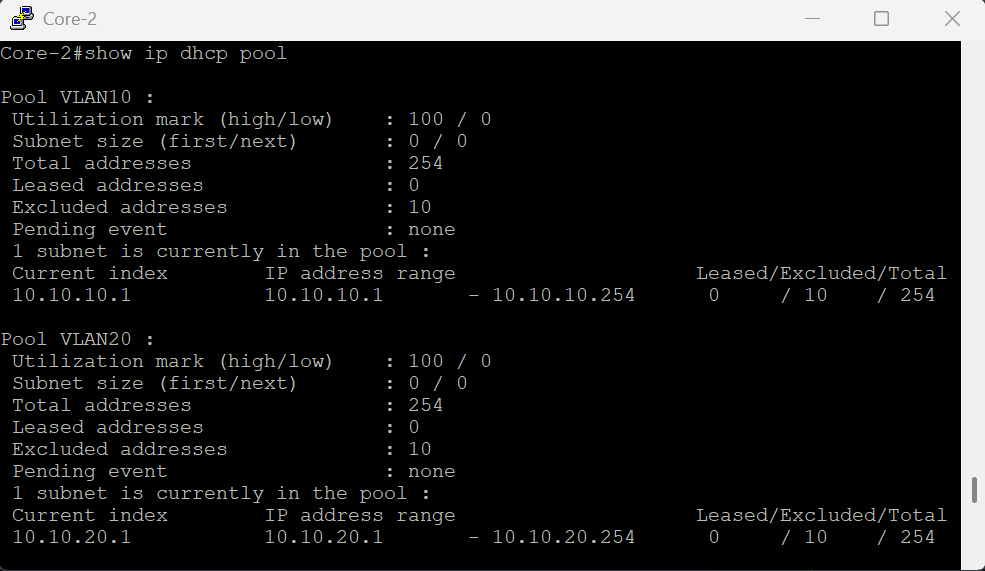
\includegraphics[width=7cm]{img/DHCP_CORE2.png}}\hfill
			\caption{Thông tin DHCP Service}
			\label{fig:Pic_1114}
\end{figure}
\begin{itemize}
    \item DHCP Serive hoạt động trên cả CORE-1 và CORE-2, nhưng không xảy ra xung đột do CORE-1 là root cho VLAN 1, 10, 20, 30; là backup cho VLAN 40, 50, 60. Trên CORE-2 ngược lại.
\end{itemize}
\subsubsection{Xem IP interface của ASAv}
\begin{figure}[H]
			\subfloat[IP Interface của ASAv1\label{fig:Pic_22}]
			{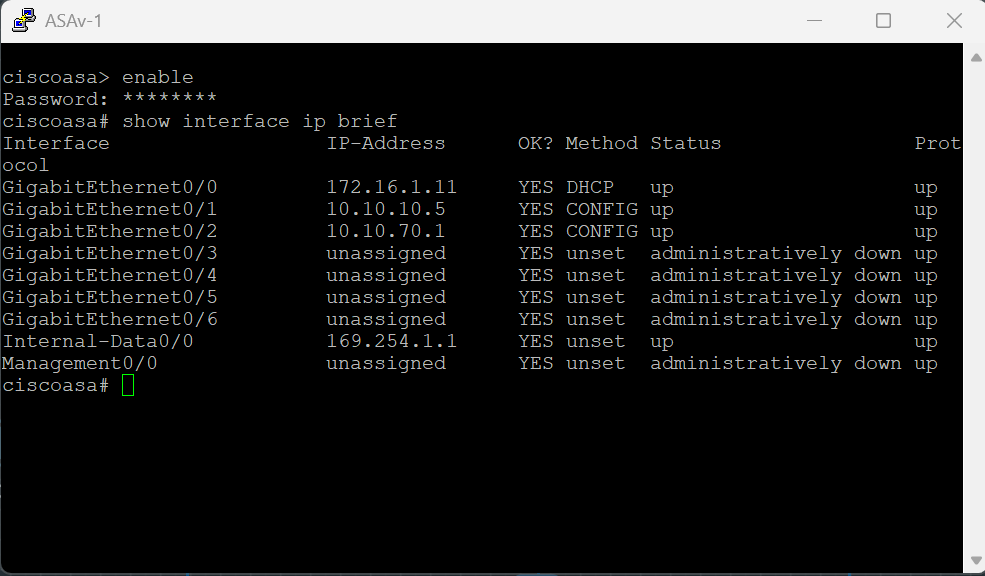
\includegraphics[width=7cm]{img/IP_ASAv1.png}}\hfill
			\subfloat[IP Interface của ASAv2\label{fig:Pic_23}]
			{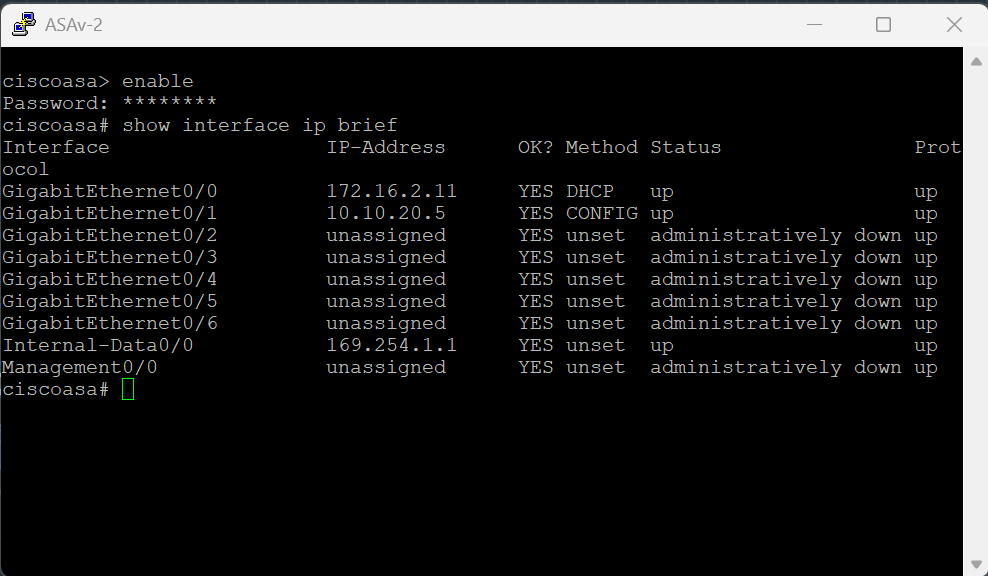
\includegraphics[width=7cm]{img/IP_ASAv2.png}}\hfill
			\caption{Xem cấu hình IP ASAv}
			\label{fig:Pic_1115}
\end{figure}
\subsubsection{Xem miền OSPF trên CORE và ASAv}
\begin{figure}[H]
			\subfloat[Miền OSPF trên CORE-1 và CORE-2\label{fig:Pic_22}]
			{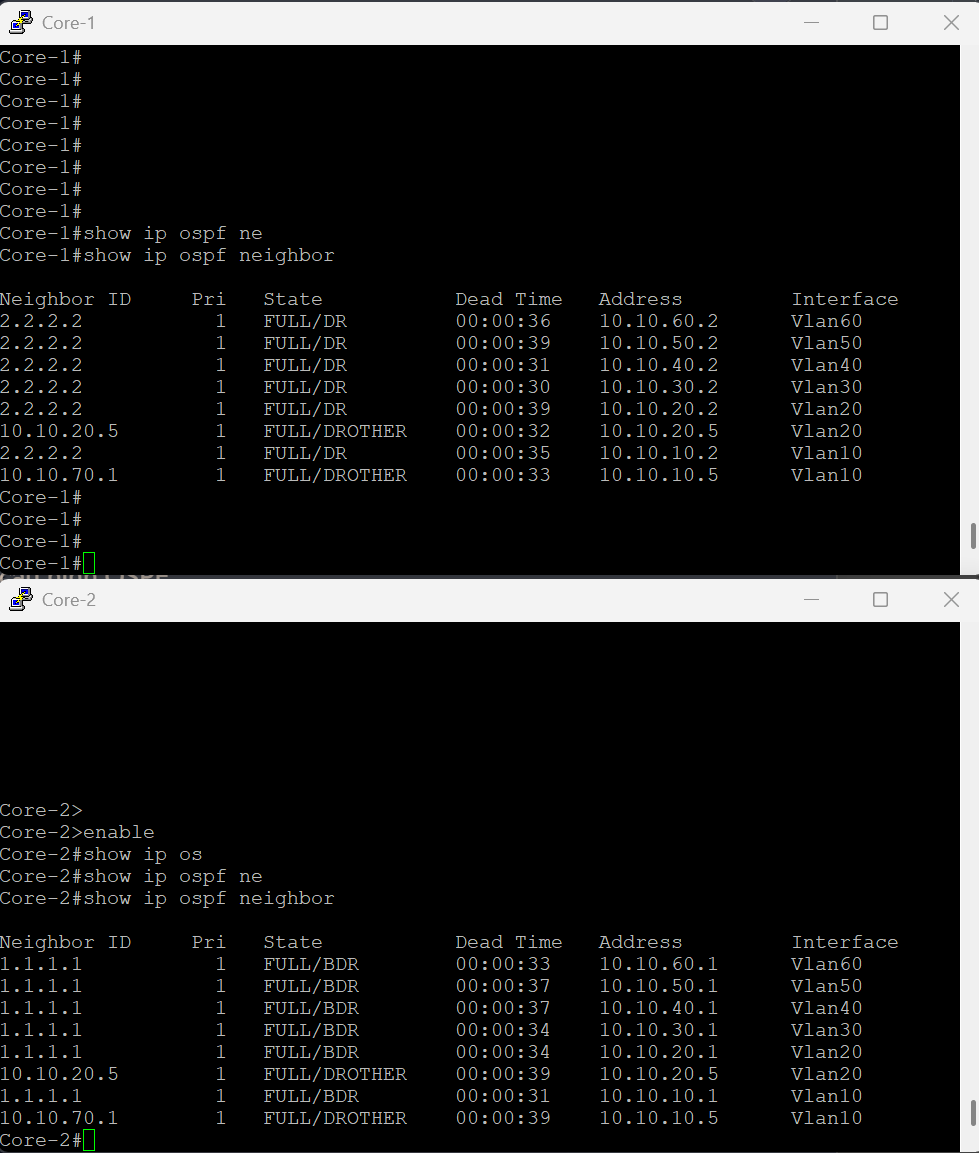
\includegraphics[width=7cm]{img/OSPFCORE.png}}\hfill
			\subfloat[Miền OSPF trên ASAv1 và ASAv2\label{fig:Pic_23}]
			{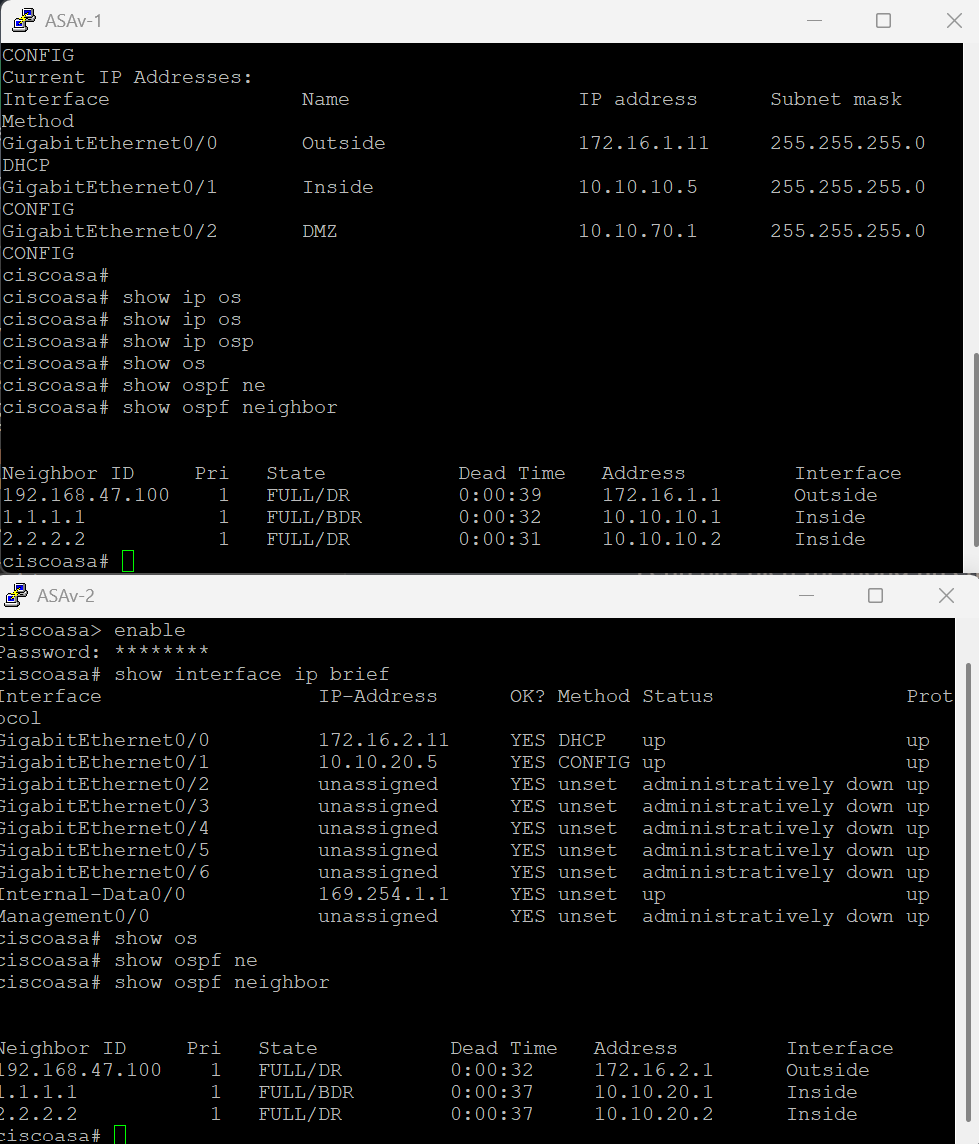
\includegraphics[width=7cm]{img/OSPFASA.png}}\hfill
            \subfloat[IP routing trên CORE-1\label{fig:Pic_23}]
			{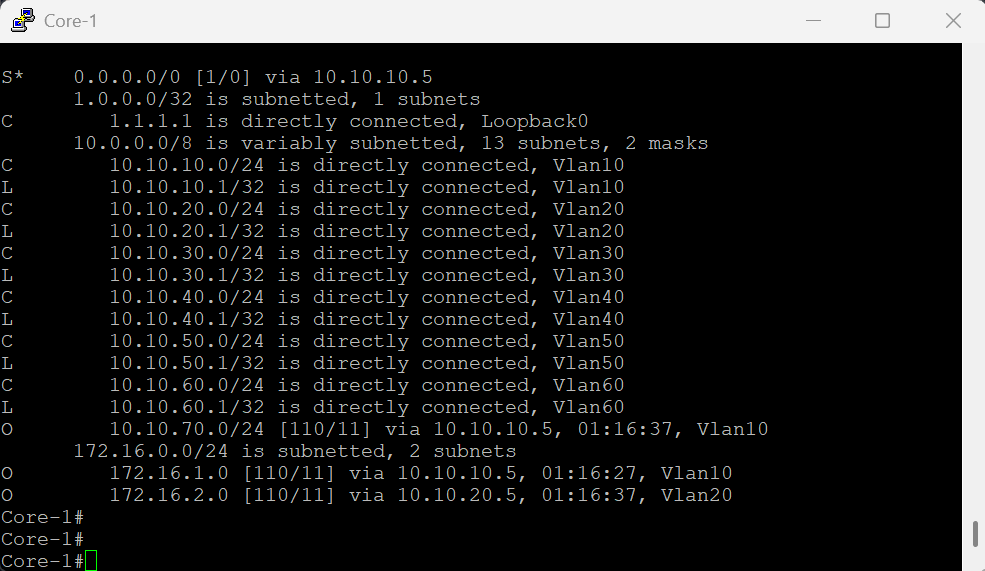
\includegraphics[width=7cm]{img/ROUTECore1.png}}\hfill
            \subfloat[IP routing trên CORE-2\label{fig:Pic_23}]
			{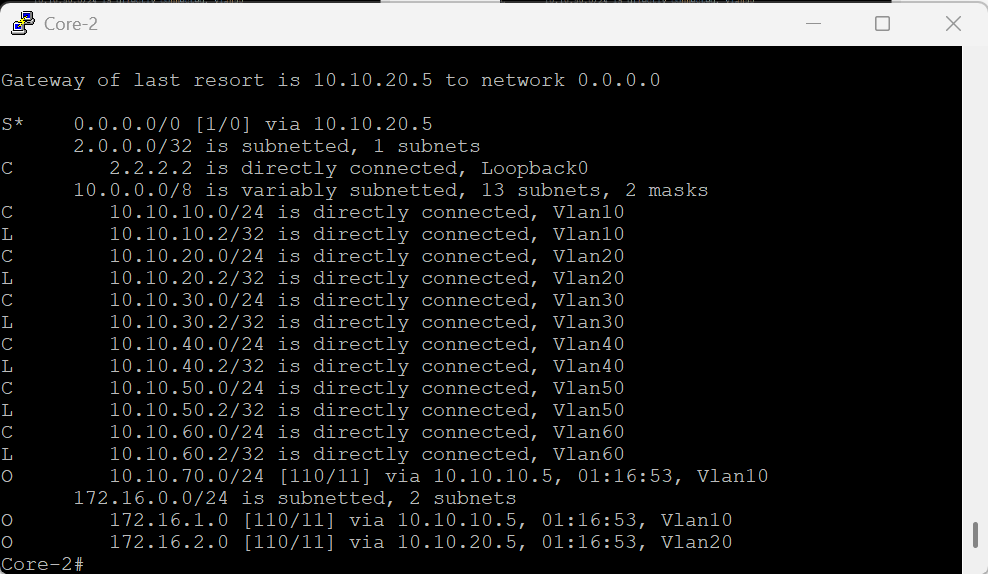
\includegraphics[width=7cm]{img/ROUTECore2.png}}\hfill
			\caption{Xem cấu hình OSPF và Routing}
			\label{fig:Pic_1116}
\end{figure}
\begin{figure}[H]
			\subfloat[IP Routing trên ASAv\label{fig:Pic_22}]
			{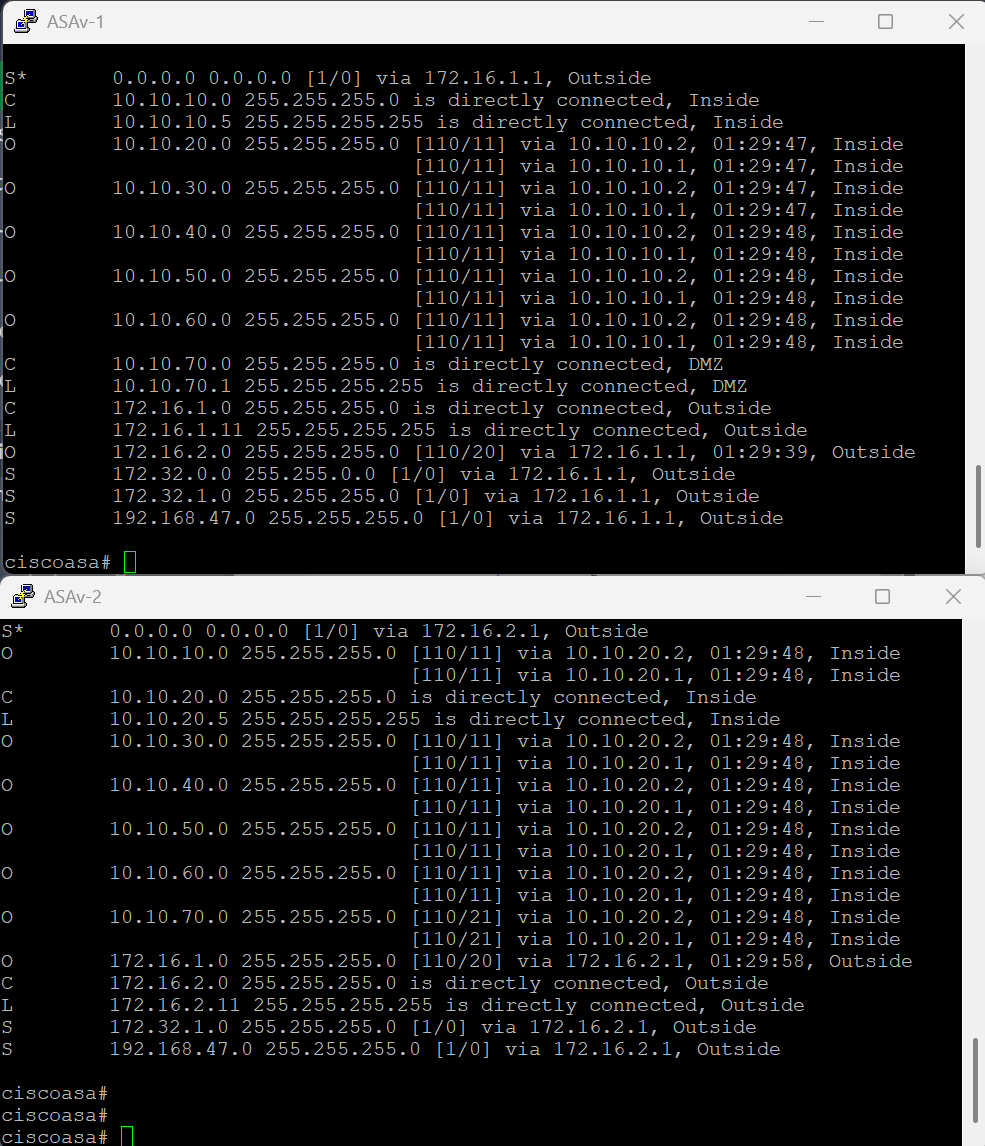
\includegraphics[width=7cm]{img/ROUTEASA.png}}\hfill
			\subfloat[IP Routing trên Router ISP\label{fig:Pic_23}]
			{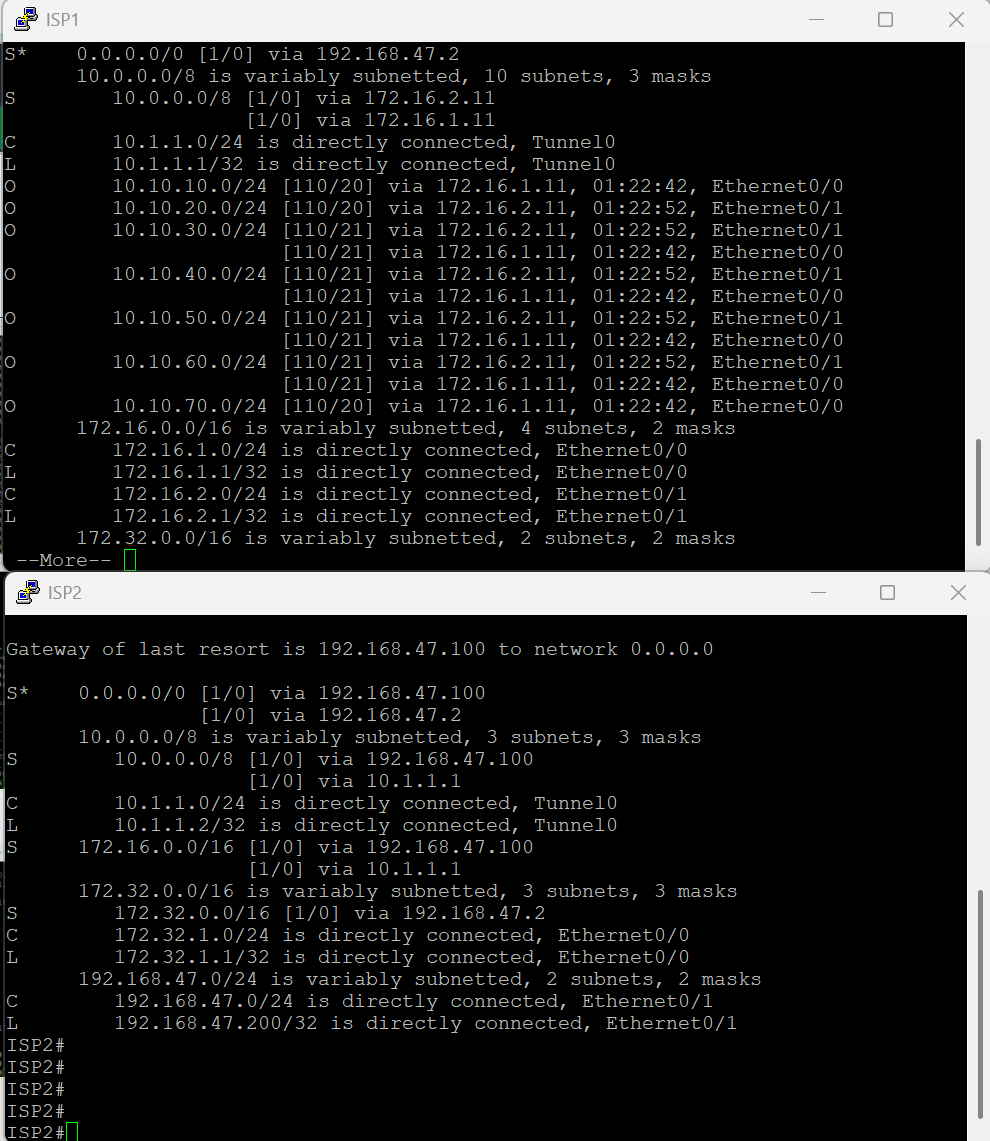
\includegraphics[width=7cm]{img/ROUTEISP.png}}\hfill
			\caption{Xem cấu hình OSPF và Routing}
			\label{fig:Pic_1117}
\end{figure}
\subsubsection{Xem cấu hình Tunnel GRE}
\begin{figure}[H]
			\subfloat[Xem cấu hình tunnel trên ISP1\label{fig:Pic_22}]
			{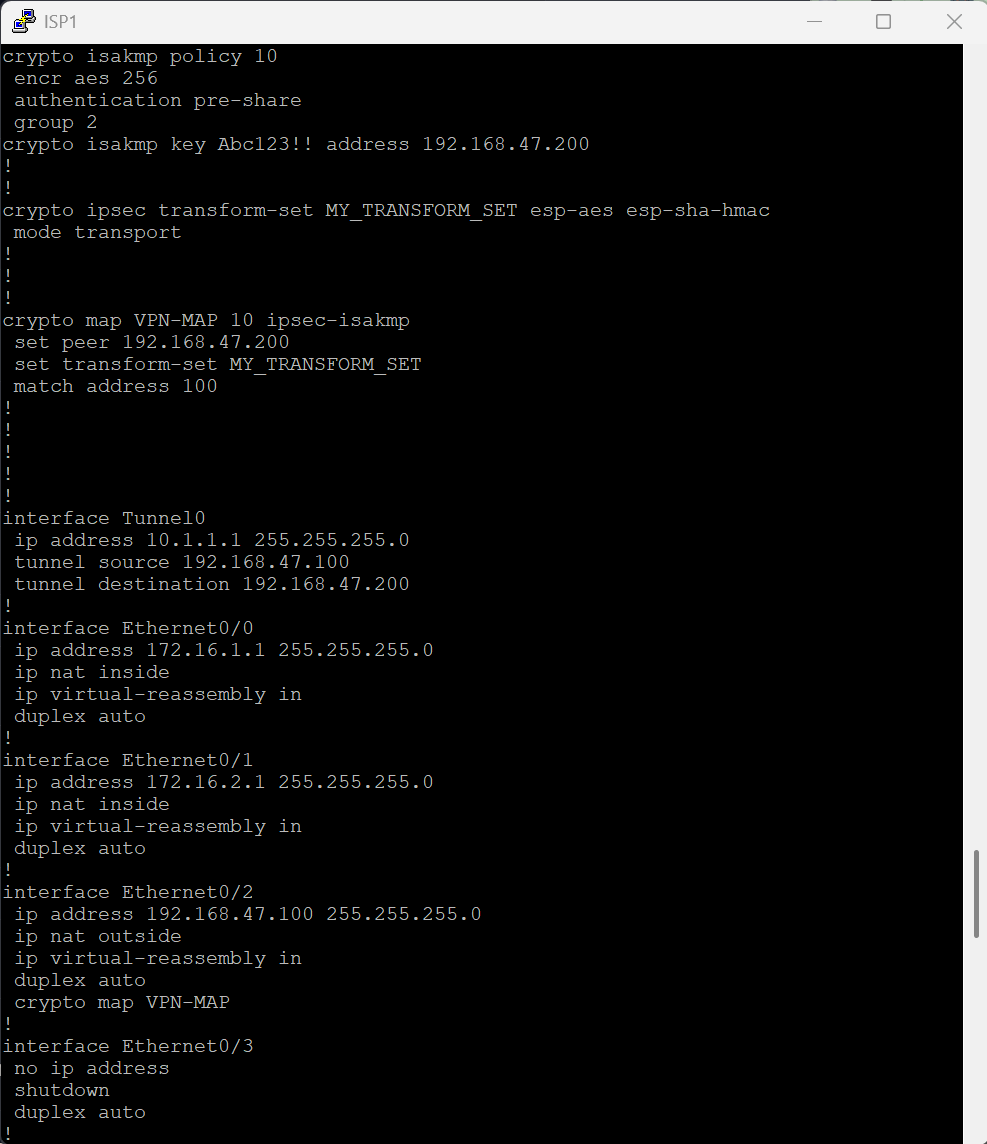
\includegraphics[width=7cm]{img/GREISP1.png}}\hfill
			\subfloat[Xem cấu hình tunnel trên ISP2\label{fig:Pic_23}]
			{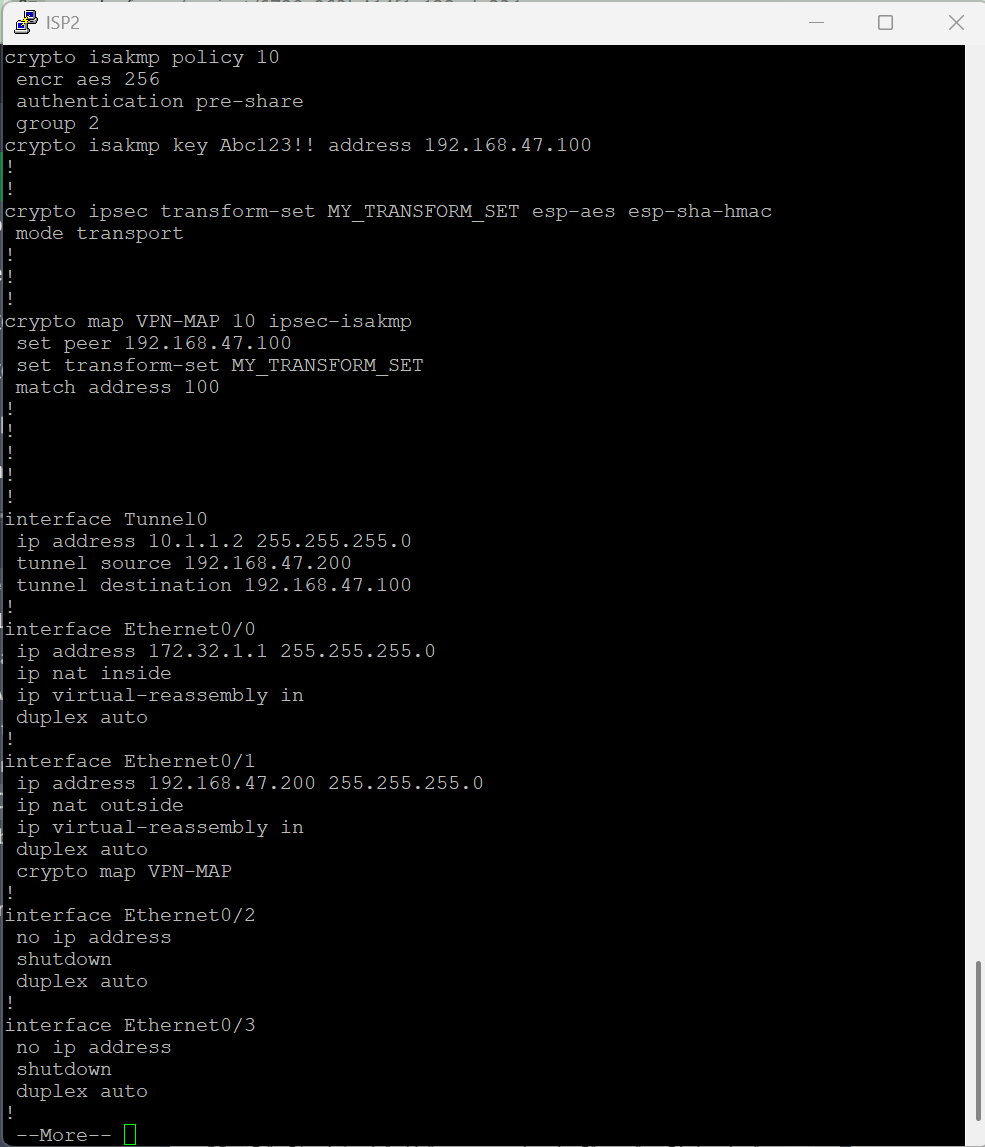
\includegraphics[width=7cm]{img/GREISP2.png}}\hfill
			\caption{Xem cấu hình đường hầm GRE Tunnel và VPN MAP}
			\label{fig:Pic_1117}
\end{figure}

\section*{4.2 Quản lý và bảo trì}
\addcontentsline{toc}{section}{4.2 Quản lý và bảo trì}
Để đảm bảo hệ thống mạng hoạt động ổn định, hiệu quả và an toàn, cần thực hiện các công việc quản lý và bảo trì định kì.

\subsection*{4.2.1 Quản lý hệ thống}
\addcontentsline{toc}{subsection}{4.2.1 Quản lý hệ thống}

\textbf{ $-$ Cấu trúc và phân vùng mạng}

\begin{itemize}[left = 2cm]
    \item Duy trì cấu hình các VLAN (10, 20, 30, 40, 50, 60) để phân đoạn mạng, cách ly lưu lượng và đảm bảo bảo mật.
    \item Kiểm tra các kết nối trunk trên switch để truyền VLAN đúng cấu hình.
    \item Theo dõi địa chỉ IP được cấp phát trong từng VLAN (10.10.x.x/24), đảm bảo không có xung đột hoặc trùng lặp.
    \item Sử dụng công cụ quản lý IP như phpIPAM để tối ưu.
\end{itemize}

\textbf{$-$ Theo dõi hiệu suất hoạt động}
\begin{itemize}[left = 2cm]
    \item Dùng công cụ như Zabbix, Nagios, hoặc PRTG để giám sát hiệu suất switch, router, firewall và đường truyền (Cat6a, cáp quang OM4).
    \item Thiết lập cảnh báo khi phát hiện sự cố như mất kết nối, cổng quá tải hoặc suy hao tín hiệu.
    \item Triển khai máy chủ syslog để thu thập nhật ký từ switch, router và firewall.
    \item Phân tích log định kỳ để phát hiện lỗi hoặc mối đe dọa bảo mật.
\end{itemize}

\textbf{$-$ Quản lý truy cập và bảo mật}
\begin{itemize}[left = 2cm]
    \item Áp dụng Access Control List (ACL) để hạn chế lưu lượng giữa các VLAN và DMZ.
    \item Kích hoạt xác thực 802.1X trên switch access để kiểm soát kết nối của thiết bị đầu cuối.
    \item Cấu hình chính sách tường lửa trên ASAv-1 và ASAv-2 để bảo vệ DMZ và mạng nội bộ khỏi truy cập trái phép.
    \item Kiểm tra các chính sách NAT và VPN nếu có.
\end{itemize}

\subsection*{4.2.2 Bảo trì hệ thống}
\addcontentsline{toc}{subsection}{4.2.2 Bảo trì hệ thống}

\textbf{$-$ Kiểm tra định kỳ}
\begin{itemize}[left = 2cm]
    \item Kiểm tra tình trạng các cổng, module quang và dây cáp (Cat6a, OM4). Xem xét trạng thái dự phòng của các kết nối giữa 2 Switch Core.
    \item Đảm bảo chính sách tường lửa được cập nhật và phù hợp với nhu cầu sử dụng.
    \item Theo dõi hiệu suất CPU, RAM của firewall để tránh quá tải.
    \item Kiểm tra các máy chủ (Web/Mail Server, Database Server) và đảm bảo dịch vụ được chạy ổn định.
\end{itemize}

\textbf{$-$ Cập nhật phần mềm và firmware}
\begin{itemize}[left = 2cm]
    \item Cập nhật firmware cho tất cả các thiết bị mạng (switch, router, firewall) để vá lỗ hổng bảo mật.
    \item Cập nhật hệ điều hành và phần mềm trên máy chủ để tránh rủi ro từ các lỗi bảo mật cũ.
\end{itemize}

\textbf{$-$ Sao lưu và khôi phục}
\begin{itemize}[left = 2cm]
    \item Sao lưu định kỳ cấu hình của tất cả các thiết bị mạng (switch, router, firewall) và lưu tại nhiều nơi an toàn.
    \item Triển khai giải pháp backup cho các máy chủ (Database Server, Web/Mail Server) để khôi phục nhanh trong trường hợp sự cố.
\end{itemize}

\textbf{$-$ Kiểm tra dự phòng và khả năng chịu lỗi}
\begin{itemize}[left = 2cm]
    \item Đảm bảo các kết nối dự phòng giữa 2 Switch Core hoạt động tốt thông qua giao thức như HSRP hoặc VRRP.
    \item Kiểm tra khả năng chuyển đổi giữa ISP1 và ISP2 khi xảy ra lỗi.
    \item Chuẩn bị các thiết bị dự phòng để sẵn sàng các thiết bị thay thế để sử dụng ngay khi cần.
\end{itemize}

\textbf{$-$ Xử lý sự cố}
\begin{itemize}[left = 2cm]
    \item Tài liệu hoá mạng: Duy trì sơ đồ mạng chi tiết để dễ dàng xác định các thành phần và kết nối khi cần xử lý sự cố.
    \item Phân loại sự cố: Xác định mức độ ưu tiên dựa trên ảnh hưởng. Ví dụ: sự cố ở Core Switch cần ưu tiên cao nhất.
    \item Hỗ trợ từ nhà cung cấp: Duy trì liên lạc với nhà cung cấp dịch vụ (ISP) và thiết bị (Cisco, Fortinet) để nhận hỗ trợ khi cần.
\end{itemize}

